%% LyX 2.3.4.2 created this file.  For more info, see http://www.lyx.org/.
%% Do not edit unless you really know what you are doing.
\documentclass[11pt,oneside,american,czech]{book}
\usepackage[T1]{fontenc}
\usepackage[utf8]{inputenc}
\usepackage[a4paper]{geometry}
\geometry{verbose,tmargin=4cm,bmargin=3cm,lmargin=3cm,rmargin=2cm,headheight=0.8cm,headsep=1cm,footskip=0.5cm}
\pagestyle{headings}
\setcounter{secnumdepth}{3}
\usepackage{url}
\usepackage{amsmath}
\usepackage{amsthm}
\usepackage{amssymb}
\usepackage{graphicx}

\usepackage{setspace}

\usepackage{pdfpages}
\usepackage[backend=bibtex]{biblatex}
\addbibresource{ref}

\makeatletter
%%%%%%%%%%%%%%%%%%%%%%%%%%%%%% Textclass specific LaTeX commands.
\newenvironment{lyxlist}[1]
	{\begin{list}{}
		{\settowidth{\labelwidth}{#1}
		 \setlength{\leftmargin}{\labelwidth}
		 \addtolength{\leftmargin}{\labelsep}
		 \renewcommand{\makelabel}[1]{##1\hfil}}}
	{\end{list}}

%%%%%%%%%%%%%%%%%%%%%%%%%%%%%% User specified LaTeX commands.
%% Font setup: please leave the LyX font settings all set to 'default'
%% if you want to use any of these packages:

%% Use Times New Roman font for text and Belleek font for math
%% Please make sure that the 'esint' package is turned off in the
%% 'Math options' page.
\usepackage[varg]{txfonts}

%% Use Utopia text with Fourier-GUTenberg math
%\usepackage{fourier}

%% Bitstream Charter text with Math Design math
%\usepackage[charter]{mathdesign}

%%---------------------------------------------------------------------

%% Make the multiline figure/table captions indent so that the second
%% line "hangs" right below the first one.
%\usepackage[format=hang]{caption}

%% Indent even the first paragraph in each section
\usepackage{indentfirst}

%%---------------------------------------------------------------------

%% Disable page numbers in the TOC. LOF, LOT (TOC automatically
%% adds \thispagestyle{chapter} if not overriden
%\addtocontents{toc}{\protect\thispagestyle{empty}}
%\addtocontents{lof}{\protect\thispagestyle{empty}}
%\addtocontents{lot}{\protect\thispagestyle{empty}}

%% Shifts the top line of the TOC (not the title) 1cm upwards 
%% so that the whole TOC fits on 1 page. Additional page size
%% adjustment is performed at the point where the TOC
%% is inserted.
%\addtocontents{toc}{\protect\vspace{-1cm}}

%%---------------------------------------------------------------------

% completely avoid orphans (first lines of a new paragraph on the bottom of a page)
\clubpenalty=9500

% completely avoid widows (last lines of paragraph on a new page)
\widowpenalty=9500

% disable hyphenation of acronyms
\hyphenation{CDFA HARDI HiPPIES IKEM InterTrack MEGIDDO MIMD MPFA DICOM ASCLEPIOS MedInria}

%%---------------------------------------------------------------------

%% Print out all vectors in bold type instead of printing an arrow above them
\renewcommand{\vec}[1]{\boldsymbol{#1}}

% Replace standard \cite by the parenthetical variant \citep
%\renewcommand{\cite}{\citep}

\makeatother

\usepackage{babel}
\begin{document}
%\def\documentdate{7. \v{c}ervence 2021}

\def\documentdate{\today}

\pagestyle{empty}
{\centering

\noindent %
\begin{minipage}[c]{3cm}%
\noindent \begin{center}

\includegraphics[width=3cm,height=3cm,keepaspectratio]{Images/TITLE/cvut}
\par\end{center}%
\end{minipage}%
\begin{minipage}[c]{0.6\linewidth}%
\begin{center}
\textsc{\large{}České vysoké učení technické v Praze}{\large{}}\\
{\large{}Fakulta jaderná a fyzikálně inženýrská}
\par\end{center}%
\end{minipage}%
\begin{minipage}[c]{3cm}%
\noindent \begin{center}

\includegraphics[width=3cm,height=3cm,keepaspectratio]{Images/TITLE/fjfi}
\par\end{center}%
\end{minipage}

\vspace{3cm}

\textbf{\huge{}Automatická registrace snímků video}{\huge\par}

\vspace{1cm}

\selectlanguage{american}%
\textbf{\huge{}Automatic registration of video
frames}{\huge\par}

\selectlanguage{czech}%
\vspace{2cm}

{\large{}Bakalářská práce}{\large\par}

}

\vfill{}

\begin{lyxlist}{MMMMMMMMM}
\begin{singlespace}
\item [{Autor:}] \textbf{Daniela Lichnovská}
\item [{Vedoucí~práce:}] \textbf{doc. Ing. Filip Šroubek, Ph.D. DSc.}
\item [{Konzultant:}] \textbf{Ing. Lukáš Tryner}
\item [{Akademický~rok:}] 2020/2021
\end{singlespace}
\end{lyxlist}
%\newpage{}

~

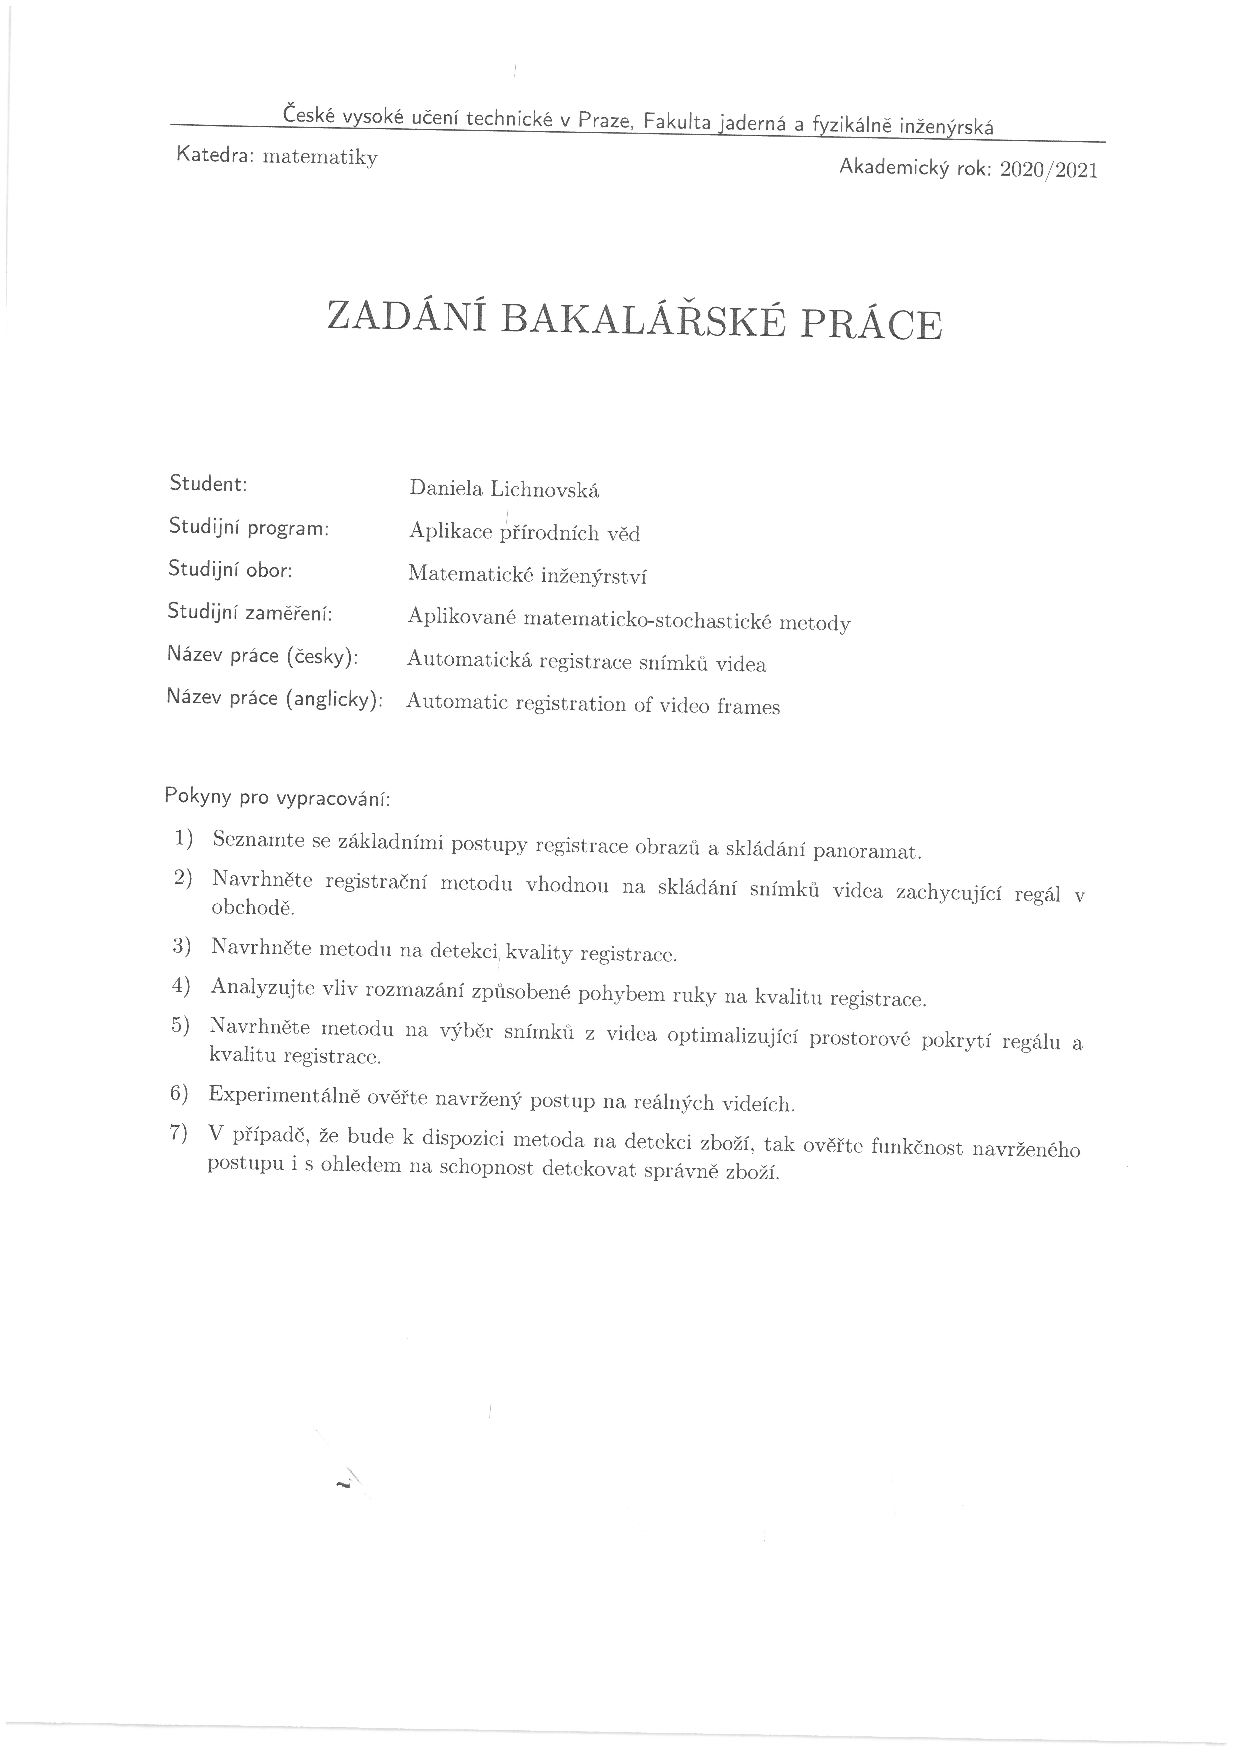
\includepdf[pages=-]{Images/zadani_cele.pdf}

%\vfill{}
%
%\begin{center}
%- Zadání práce -
%\par\end{center}
%
%\vfill{}
%
%~\newpage{}
%
%~
%
%\vfill{}
%
%\begin{center}
%- Zadání práce (zadní strana) -
%\par\end{center}
%
%\vfill{}

%~\newpage{}

\noindent \emph{\Large{}Poděkování:}{\Large\par}

\noindent Chtěl bych zde poděkovat především svému školiteli ...................
za pečlivost, ochotu, vstřícnost a odborné i lidské zázemí při vedení
mé diplomové práce. Dále děkuji svému konzultantovi ................
za ................

\vfill

\noindent \emph{\Large{}Čestné prohlášení:}{\Large\par}

\noindent Prohlašuji, že jsem tuto práci vypracoval samostatně a uvedl
jsem všechnu použitou literaturu.

\bigskip{}

\noindent V Praze dne \documentdate\hfill{}Daniela Lichnovská

\vspace{2cm}

\newpage{}

\begin{onehalfspace}
\noindent \emph{Název práce:}

\noindent \textbf{Název práce}
\end{onehalfspace}

\bigskip{}

\noindent \emph{Autor:} Daniela Lichnovská

\bigskip{}

\noindent \emph{Obor:} Matematické inženýrství\bigskip{}

\noindent \emph{Zaměření:} Aplikované matematicko-stochaistické metody

\bigskip{}

\noindent \emph{Druh práce:} Bakalářská práce

\bigskip{}

\noindent \emph{Vedoucí práce:} doc. Ing. Filip Šroubek, Ph.D. DSc.,
ÚTIA AV ČR Praha, v.v.i.,
Pod Vodárenskou věží 4,
182 00 Praha 8

\bigskip{}

\noindent \emph{Konzultant:} Ing. Lukáš Tryner,
DataSentics, a.s.,
Washingtonova 1599/17,
Praha 1

\bigskip{}

\noindent \emph{Abstrakt:} Abstrakt max. na 10 řádků. Abstrakt max.
na 10 řádků. Abstrakt max. na 10 řádků. Abstrakt max. na 10 řádků.
Abstrakt max. na 10 řádků. Abstrakt max. na 10 řádků. Abstrakt max.
na 10 řádků. Abstrakt max. na 10 řádků. Abstrakt max. na 10 řádků.
Abstrakt max. na 10 řádků. Abstrakt max. na 10 řádků. Abstrakt max.
na 10 řádků. Abstrakt max. na 10 řádků. Abstrakt max. na 10 řádků.
Abstrakt max. na 10 řádků. Abstrakt max. na 10 řádků. Abstrakt max.
na 10 řádků. Abstrakt max. na 10 řádků. Abstrakt max. na 10 řádků.
Abstrakt max. na 10 řádků. Abstrakt max. na 10 řádků. Abstrakt max.
na 10 řádků. Abstrakt max. na 10 řádků. Abstrakt max. na 10 řádků.
Abstrakt max. na 10 řádků. Abstrakt max. na 10 řádků. Abstrakt max.
na 10 řádků. Abstrakt max. na 10 řádků. Abstrakt max. na 10 řádků. 

\bigskip{}

\noindent \emph{Klíčová slova:} klíčová slova (nebo výrazy) seřazená
podle abecedy a oddělená čárkou

\vfill{}
~

\selectlanguage{american}%
\begin{onehalfspace}
\noindent \emph{Title:}

\noindent \textbf{Automatic registration of video frames}
\end{onehalfspace}

\bigskip{}

\noindent \emph{Author:} Daniela Lichnovská

\bigskip{}

\noindent \emph{Abstract:} Max. 10 lines of English abstract text.
Max. 10 lines of English abstract text. Max. 10 lines of English abstract
text. Max. 10 lines of English abstract text. Max. 10 lines of English
abstract text. Max. 10 lines of English abstract text. Max. 10 lines
of English abstract text. Max. 10 lines of English abstract text.
Max. 10 lines of English abstract text. Max. 10 lines of English abstract
text. Max. 10 lines of English abstract text. Max. 10 lines of English
abstract text. Max. 10 lines of English abstract text. Max. 10 lines
of English abstract text. Max. 10 lines of English abstract text.
Max. 10 lines of English abstract text. Max. 10 lines of English abstract
text. Max. 10 lines of English abstract text. Max. 10 lines of English
abstract text. Max. 10 lines of English abstract text. Max. 10 lines
of English abstract text. Max. 10 lines of English abstract text.
Max. 10 lines of English abstract text. Max. 10 lines of English abstract
text. Max. 10 lines of English abstract text.

\bigskip{}

\noindent \emph{Key words:} keywords in alphabetical order separated
by commas

\selectlanguage{czech}%
\newpage{}

\pagestyle{plain}

\tableofcontents{}

\newpage{}

\chapter*{Úvod}

\addcontentsline{toc}{chapter}{Úvod}

Text úvodu....

\chapter{Registrace obrazu}
\pagestyle{headings}
\subsection{co to je}
Registrace obrazu je proces kombinování dvou a více snímků pořízených z odlišných pohledů, času nebo zdrojů do jednoho souřadného sytému \cite{ir_survey}. Je například často používaná při zpracovávání dat ze satelitů,v počítačovém vidění nebo medicíně.

Registraci lze rozdělit do čtyř kroků:
\begin{enumerate}
\item detekce příznaků
\item korespondence příznaků
\item odhad transformace
\item transformace snímku
\end{enumerate}

\section{Detekce příznaků}
\subsection{Metoda SURF}
\subsection{Extrakce příznaků}
\section{Korespondence příznaků}
\section{Estimace modelu transformace}

\subsection{Affiní tr}
\subsection{Projektivní tr}
\section{resamplovaní}
\section{pipeline}

\chapter{Výběr snímků z videa}


\pagestyle{headings}

\section{focus measure}
[https://www.pyimagesearch.com/2015/09/07/blur-detection-with-opencv/]

Nejkvalitnější snímky z videa jsou ty s nejmenším rozmazáním. Méně rozmazaný snímek zároven zřejmě bude mít výraznější hrany než ten více rozmazaný. Hrany detekujeme pomocí konvoluce Laplaceova operátoru s vybraným snímkem. Výsledný (absolutní) průměr této matice nám bude sloužit jako nástroj k porovnávání rozmazání mezi snímky. Tato metoda není úplně přesná, protože se scéna na snímcích konstantě mění, nicméně se nemění tak dramaticky, aby nebyla použitelná.
\section{Velikost okna}
Předpokládáme rychlost kamery 20 cm/s a frame rate 30FPS ,tedy posun 2/3 cm/frame. Chceme aby se dva snímky překrývali alespon ze 1/3 (při menším překryvu by počítání tr.mat mohlo být obtížné/nepřesné) a zároven se nepřerývali více než ze 1/2 (minimalizace počtu snímků). Předpokládáme, že snímek zobrazuje vertikálně 1 m ve skutečnosti. Pak se dostáváme na hodnotu okna 37-75 framů.

Nápad : Počítání rychlosti kamery. 2 kola

1) Vyberu dostatečně ostré snímky (jen na začátku/ celé video?). Možná budu potřebovat pevné okno?
2) Spočítám si projektivní tr. matice.
3) Pomocí velikosti posunu tr.matice a časovou vzdáleností spočítám průměrnou rychlost.
4) Přes známou rychlost spočítám přesnější okno

100 frameu uprostred-spocitam rychlost z toho dynamicke zvetsivano/zmensovani okna podle predchoziho-lepsi

\section{Error threshold}
Pro odhad dobré transformace použijeme následující metodu: Označíme smer. odchylku intenzity snímku jako errThresh. Tato hodnota nám bude sloužit jako prah při porovnávání s chybou transformace. Ta je spočítána jako sum(abs(I1-I2)) kde I1,I2 jsou překrývající se části snímků. Pokud se chyba žádného snímku nevejde pod ErrThresh, je vybrán snímek s nejmenší chybou transformace v daném okně.

$mean = sum(x)/length(x)$

$variance = sum((x - mean(x)).^2)/(length(x) - 1)$

$std = sqrt(variance)$
\section{pipeline}
,Pro všechny snímky ve videu je spočítána focus measure. Všechny ostatní práce se snímky je postupně dělána ve vyhrazených oknech, což je soubor snímků vzdálený od předchozího vybraného snímku minimální a maximální vzáleností(vzdáleností je myšleno časové pořadí snímků). Pro první průchod je jednoduše vybrán snímek s největší fm a spočítán ErrThresh pomocí něj. Zbytek cyklu probíhá takto:

1) Všechny snímky okna jsou v sestupném pořadí seřazeny podle jejich focus measure.

2) Snímky jsou jeden po druhém registrovány na vybraný snímek z předchozího okna, dokun není nalezen snímek s chybou transformace menší než ErrThresh. Pokud ani jeden není menší, je vybrán snímek s nejmenší chybout tr.

3) Tento snímek je přidán do konečného výběru snímků 
\chapter{Registrace panoramatu}
[https://www.mathworks.com/help/vision/ug/feature-based-panoramic-image-stitching.html]
\section{computeTforms}

Transfromační matice jsou počítány následující způsobem: Snímek je převeden do černobílý (1 vrstva místo 3 u RGB) a jsou naněm detekovány body pomocí SURF detektoru. Z těchto bodů jsou vybrány příznaky, které jsou následně spárovány s příznaky z předchozího snímku. Tyto 2 seznamy jsou poté použity funkcí estimateGeometricTransform, která spočítá odpovídající tr. matici. Pro potřeby panoramatu je použita affiní transformace, protože u projektivní dochází při součinu matic ke velké chybě.

Pokud chceme, aby referenčním snímkem v panoramatu byl jiný než první, je potřeba je přepočítat pomocí tforms(j).T = tforms(j).T * Tinv.T; kde Tinv je inverze ref. snímku.
\section{computeLimits}

Je třeba znát rozměry výsledného panoramatu, čehož docílíme transformací 4 bodů okrajů u všech snímku a následným výběrem těch nejzaších. V tomto kroce je dobré ověřit velikost pro výsledné panorama, pokud je příliš velká, evidentně někde nastala chyba.
\section{createPanorama}

Díky znalosti rozměrů panoramatu si můžeme vytvořit konečný souřadný systém, do kterého nejdříve vložíme masku (opět 4 kraje původního snímku) a následně do místa masky vložíme transformovaný snímek. (Masku pak můžeme využít na zobrazení vizualizaci poskládání všech snímků)
\section{Omezení}

Jak bylo výše uvedeno, u dlouhých panoramat s jakými pracujeme my, je třeba použít affiní, či podobnostní transformaci, nebot při součinu projektivních transformací dochází ke stále větší a větší chybě, a při více než 5-7 snímcích ani nelze žádné panorama vytvořit.
\chapter{Experimenty}
\pagestyle{headings}
\section{Opakovatelnost(repeatability)}

\begin{figure}
  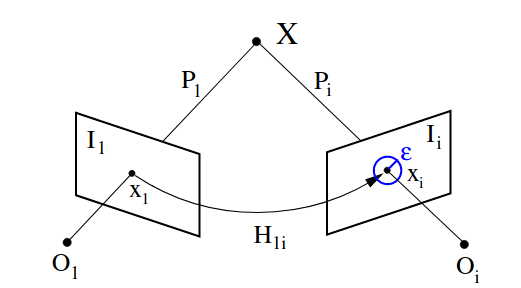
\includegraphics[width=\linewidth]{Images/aaa.png}
  \caption{Ilustrace principu opakovatelnosti}
  \label{fig:repeatabil}
\end{figure}

Opakovatelnost je podle \cite{repeat} definována jako schopnost detekovat příznaky nezávisle
na změnách ve snímacích podmínkách, jako je třeba posun kamery nebo zhoršení kvality obrazu.

rep rate jako počet stejných bodů vyskytujících se na obou snímcích vzhledem k celkovém počtu detekovaných bodů. Z detekovaných bodů vybíráme pouze ty, které jsou součástí scény vyskytujících se na obou snímcích.

Je důležité vzít v úvahu nepřesnost detekce. Korespondující bod se nebude nacházet přesně daném místě určeném maticí, ale v jeho eps
-okolí. eps-reapeatabilitu definujeme jako:
 $$Ri(eps) = {(xi,xj)|dist(Hijxi, xj) < eps}$$

Počet detekovaných bodů ve společné části snímku nebude stejný, proto vybereme menší z nich, abychom zajistili existenci bodu z eps
-reapeatability. Repeatability rate je tedy definováno následovně: 
$$ri(eps)=abs(Ri(eps))/min(ni,j)$$


\section{Vliv rozmazání na registraci}
Pro sledování vlivu rozmazání na kvalitu registrace použijeme dvojice sousedících snímků, které uměle rozmažeme aplikací motion-blur filtru náhodné orientace v rozsahu <0,190> a pevně zvolené délky v rozsahu <1,50>, kdy je postupně přidávana po inkrementech 5(pixelů?). Z jedné dvojice tak získáme 11 (12 s originálními) párů rozmazaných snímků. U nich pak najdeme příznaky, namatchujeme je a odhadneme homografní matici. Pro E v Eps-repeatabilite dosadíme 10. Takte získáme repeatability rate.

Dále chceme znát localization error, tedy průměrnou vzdálenost bodu predikovaného tr. maticí od místa, kde se bod skutečně nachází. To se dá vyjádřit jako: 
$$dist(i) = norm(p2(i,:)-predicted(i,:)); mean(dist)$$

Takto projdeme celý daný set snímků. Tady je graf setu 1:

Na vertikální ose je repeatability rate a jeho rozptyl, na horizontální délka filtru. Jak lze vidět z grafu, do cca 30 pixelu je kvalita registrace poměrně spolehlivá, pak ale začne rychle klesat. 
\section{vliv artefaktů}
Sledování vlivu zmenšování datového toku kvalitu registrace. Plánovaný postup:

1)Vygeneruju set videí se různým datovým tokem

2)Problém s výběrem snímku (od nějakého to už nezvládne vybrat snímek)

řešení: vybírám předem dané snímky (znám čísla z originálu)

3)Dále postup stejný jako u bluru (detekce příznaků, matching, estimateGeometricTransform,etc...))
\chapter{Detekce cenovek}
\pagestyle{headings}
V této části si ukážeme využití výše zmíněných metod na problému počítání cenovek. V podstatě jde o schopnost detekce stejného objektu na více snímcích a následném rozdělění tak, aby každý snímek měl "své" cenovky. Pro toto je využití vlastností transfromačních matic ideální.

Pro samotnou detekci cenovek byla využita typ síte YOLOv5[https://github.com/ultralytics/yolov5] natrénována na cenovky od firmy DataSentics. Ta vyniká především pro svou rychlost i malou velikost, čímž je vhodná pro využití v mobilních zařízeních. Vstupem je snímek a výstupem list souřadnic bounding boxů.

Snímky jsou získany z videa postupem výše uvedeném. Mezi těmito snímky je spočítany matice projektivní transformace a je také (odděleně) vygenerováno panorama pomocí affiní transformace. Toto panoram slouží k ručnímu sčítání cenovek.

V každém cyklu jsou vzaty 3 po sobě jsoucí snímky, v nichž jsou následně detekovány cenovky. První a třetí bboxy jsou převedeny transformací do souřadného systému druhého snímku. Poté jsou přes Python knihovnu Shapely[] souřadnice bboxů převedeny do polygonů pro snadnější manipulaci.

Polygony prvního a druhého snímku jsou dávány přes sebe a pokud je nalezen překryv, polygon je odstraněn z list ve 3. a zůstává pouze ve 1. Následně jsou podobným způsoben kontrolovány polygony prvního a druhého a třetího a druhého Při nalezení překryvu ale o tom, ze kterého listu bude polygon smazán rozhoduje velikost obsahu cenovky.

Po prvním cyklu neprochází již detekované snímky sítí znovu, místo toho jsou brány seznamy z předchozích 2 cyklů. Díky tomu nedochází k duplikaci cenovek na různých snímcích. Mohlo by v nějakých případech dojít k duplikaci, pokud by se objekt objevil na 4 a více snímcích po sobě, nicméně k tomu v podstatě nedochází, vzhledem k tomu že snímky jsou vybrány z videa, tak, aby neměly tak velký překryv. Nehledě na to, že při součinu projektivních transformačních matic se rychle kumuluje chyba po několika cyklech by se bboxy přestaly překrývat.
\section{Omezení}

Sít má problém s cenovkami velmi blízko u sebe a najde neexistující cenovky. Také má problém správně detekovat cenovky vyloženě přes sebe a neobvyklých formátů(elektronické, moc dlouhé)
\section{Výsledky}

\begin{table}	
	\begin{tabular}{l|lllll}
		Číslo setu         & 1 & 2 & 3 & 4 & 5 \\ \hline
		Sečteno ručně      & 188 & 190 & xxx & xxx &  xxx\\
		Sečteno programem & 102 & 96 & xxx & xxx & xxx
	\end{tabular}
	\caption{TABLETABLETABLE.}
	\label{tab:label}
\end{table}

\begin{figure}
  \includegraphics[width=\linewidth]{Images/set30.png}
  \caption{Zobrazení cenovek na panaromatu z vid30.}
  \label{fig:price_set30}
\end{figure}


\begin{figure}
  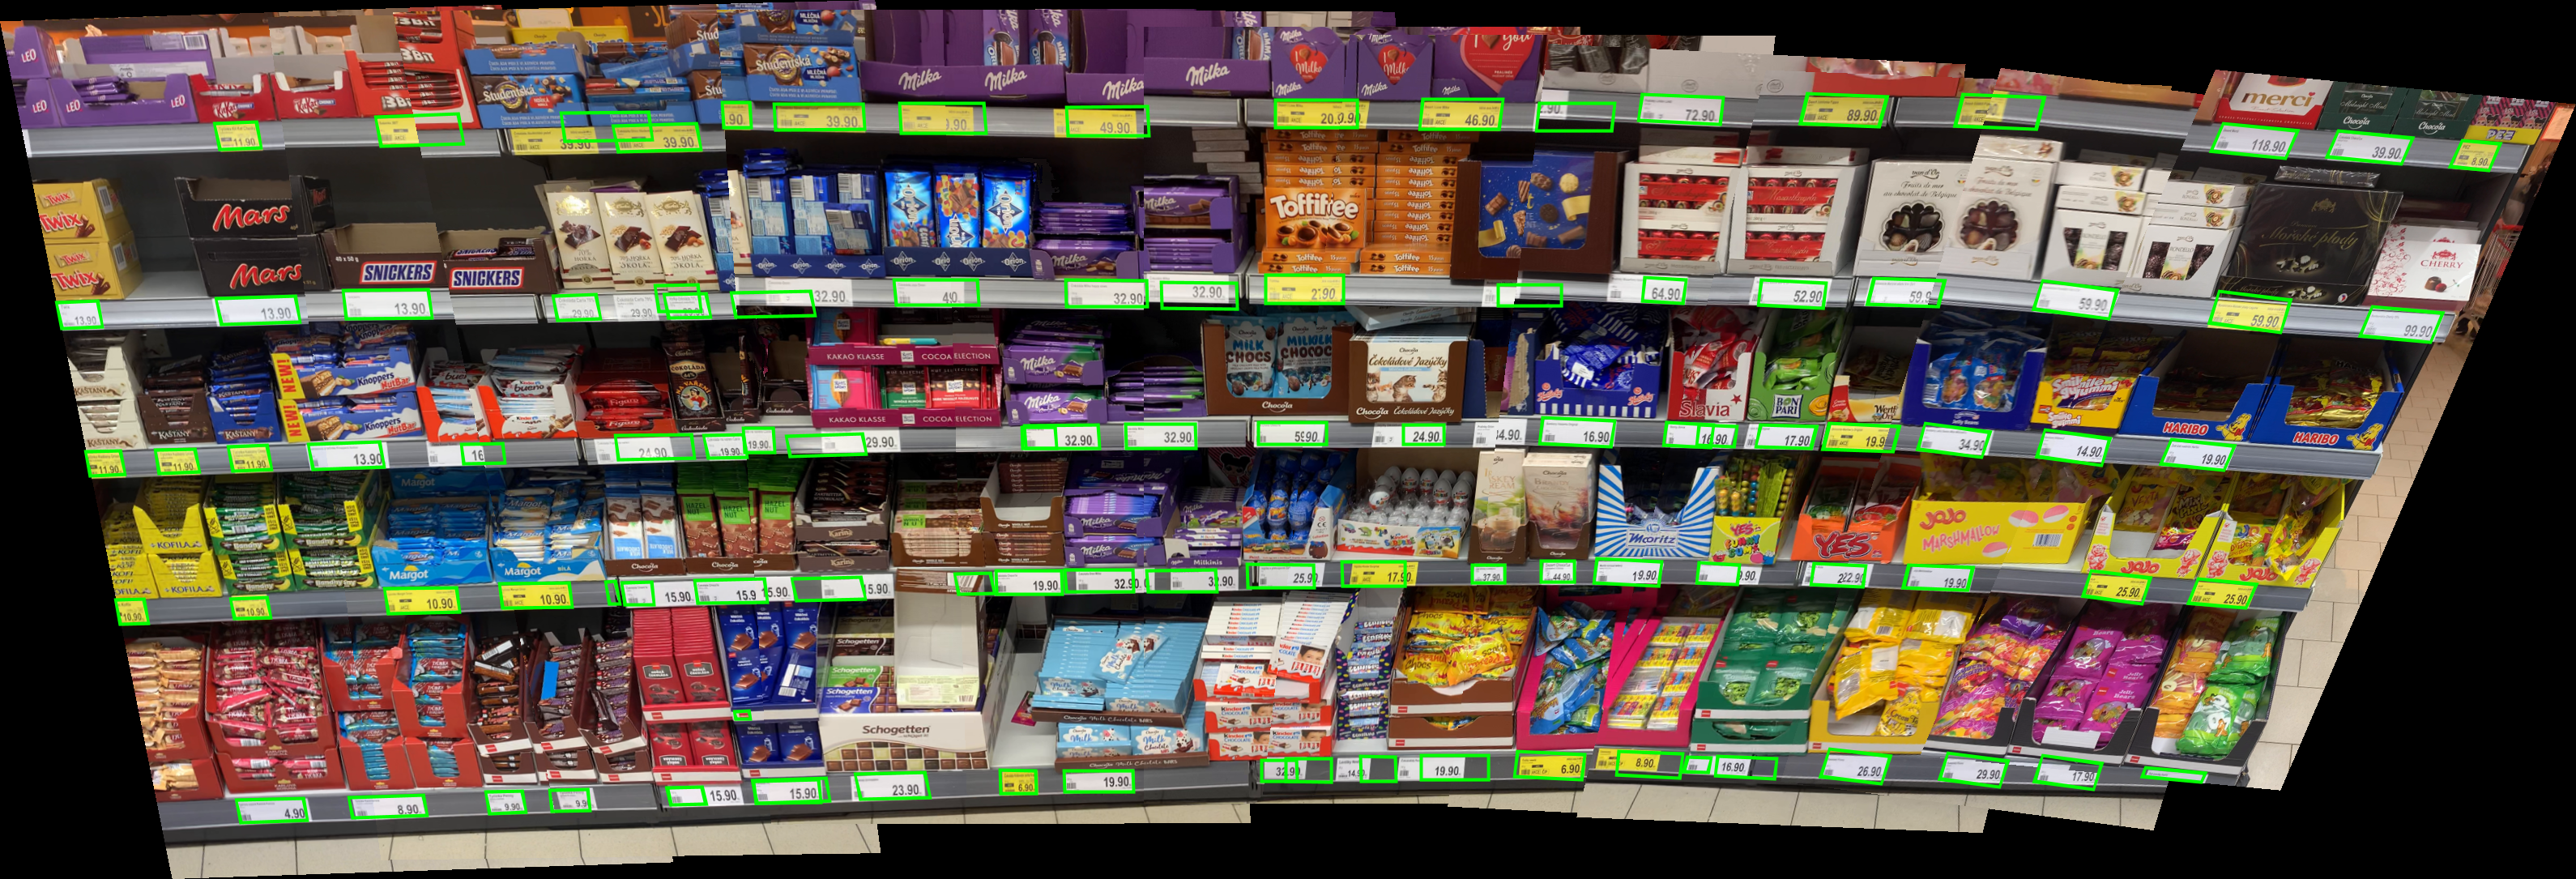
\includegraphics[width=\linewidth]{Images/set34.png}
  \caption{A boat.}
  \label{fig:price_set34}
\end{figure}





\chapter*{Závěr}

\pagestyle{plain}

\addcontentsline{toc}{chapter}{Záv\v{e}r}

Text závěru....

\printbibliography
\listoffigures
\listoftables

\end{document}
